\documentclass[a4paper,10pt]{article}

% ---------- FIXED ISSUES ----------
\setlength{\headheight}{15.5pt}    % Fix fancyhdr warning
\setlength{\marginparwidth}{2.5cm} % Fix todonotes warning

% ---------- PACKAGES ----------
\usepackage{geometry}    % Adjust page margins
\geometry{left=2.5cm, right=2.5cm, top=3cm, bottom=3cm}

\usepackage{graphicx}    % Images
\usepackage{hyperref}    % Hyperlinks
\usepackage{xcolor}      % Colors
\usepackage{listings}    % Code formatting
\usepackage{amsmath}     % Math equations
\usepackage{booktabs}    % Better tables
\usepackage{caption}     % Better figure captions
\usepackage{subcaption}  % Subfigures support
\usepackage{fancyhdr}    % Header and footer customization
\usepackage{titlesec}    % Better section titles
\usepackage{enumitem}    % Custom lists
\usepackage{minted}      % Highlighted code blocks
\usepackage{float}       % Better figure placement
\usepackage{helvet}      % Use Helvetica (Arial-like font)
\renewcommand{\familydefault}{\sfdefault} % Set default font to sans-serif

% ---------- COLOR SCHEME ----------
\definecolor{darkblue}{HTML}{1F3B4D}    % Dark Navy Blue (Headers)
\definecolor{lightgray}{HTML}{F5F5F5}   % Light Gray (Code Background)
\definecolor{darkgray}{HTML}{4D4D4D}    % Dark Gray (Text)
\definecolor{codeblue}{HTML}{007AFF}    % Blue (Keywords)
\definecolor{codegreen}{HTML}{34C759}   % Green (Strings)
\definecolor{codepurple}{HTML}{AF52DE}  % Purple (Functions)

% ---------- HEADER & FOOTER ----------
\pagestyle{fancy}
\fancyhf{}

\fancyhead[L]{\textbf{\textcolor{darkblue}{GRIB2 Processing and Visualization}}}
\fancyhead[R]{\textcolor{darkgray}{Louis Dreyfus Company - Data Team}}

% Extend the header rule to full width
\renewcommand{\headrulewidth}{1pt}  
\renewcommand{\headrule}{
    \hrule width \headwidth height 1pt
}

\fancyfoot[C]{\textcolor{darkgray}{\thepage}}

% ---------- LISTINGS SETUP ----------
\lstset{
    language=Python,
    basicstyle=\ttfamily\footnotesize\color{darkgray},
    keywordstyle=\bfseries\color{codeblue},
    stringstyle=\color{codegreen},
    commentstyle=\color{darkgray},
    identifierstyle=\color{codepurple},
    breaklines=true,
    frame=single,  % Ensures code is in a proper box
    numbers=left,
    numberstyle=\tiny\color{gray},
    backgroundcolor=\color{lightgray},
    rulecolor=\color{darkblue},
    xleftmargin=15pt,  % Proper margin alignment for Overleaf
    framexleftmargin=10pt
}

\begin{document}

% ---------- TITLE PAGE ----------
\begin{titlepage}
    \centering
    
\includegraphics[width=0.4\textwidth]{dreyfus_logo.jpg}

    \vspace{2cm}
    {\LARGE\textbf{\textcolor{darkblue}{LOUIS DREYFUS COMPANY}}} \\
    \vspace{0.5cm}
    {\Large\textcolor{darkgray}{Data Engineer Test - GRIB2 File Manipulation}}

    \vfill
    {\LARGE \sffamily \textbf{Pedro Mendes}} \\
    {\large petter.mendes@outlook.com}
    

    \vspace{1.5cm}
    {\large \textcolor{darkgray}{\today}}
\end{titlepage}

% ---------- ABSTRACT ----------
\begin{abstract}
This document presents a structured approach to processing and visualizing GRIB2 meteorological data using Python. The workflow includes \textbf{data loading, transformation, visualization, and GIS integration}. This structured methodology ensures efficiency when handling large datasets while maintaining data integrity.
\end{abstract}

% ---------------------------------------------------
% CONFIGURE LOGGING
% ---------------------------------------------------
\section{Configure Logging}
Logging is essential for debugging, monitoring, and maintaining execution transparency in a data processing workflow.

\begin{itemize}
    \item \textbf{Library Used:} \href{https://docs.python.org/3/library/logging.html}{logging}
    \item \textbf{Purpose:} Tracks processing stages and captures warnings/errors.
    \item \textbf{Custom Formatter:} Uses colors for different log levels.
\end{itemize}

\begin{minted}[
    frame=single, 
    bgcolor=lightgray, 
    fontsize=\footnotesize, 
    breaklines=true, 
    breakanywhere=true
]{python}
import logging
import colorama

# Define log styles
class ColorFormatter(logging.Formatter):
    def format(self, record):
        level_colors = {
            logging.DEBUG: "[DEBUG]",
            logging.INFO: "[INFO]",
            logging.WARNING: "[WARNING]",
            logging.ERROR: "[ERROR]",
            logging.CRITICAL: "[CRITICAL]",
        }
        log_msg = super().format(record)
        return f"{level_colors.get(record.levelno, '[LOG]')} {log_msg}"

# Configure logging
console_handler = logging.StreamHandler()
console_handler.setFormatter(ColorFormatter("%(asctime)s - %(levelname)s - %(message)s"))
logging.basicConfig(level=logging.DEBUG, handlers=[console_handler])
\end{minted}

% ---------------------------------------------------
% PART 1 - FILE EXPLORATION & METADATA EXTRACTION
% ---------------------------------------------------
\section{File Exploration and Metadata Extraction}
\textbf{Goal:} Identify and extract metadata from GRIB2 files.

\begin{itemize}
    \item \textbf{Library Used:} \href{https://docs.python.org/3/library/glob.html}{glob} for file management.
    \item \textbf{Key Metadata:} Forecast initialization time, step size, and valid times.
\end{itemize}

\begin{minted}[
    frame=single, 
    bgcolor=lightgray, 
    fontsize=\footnotesize, 
    breaklines=true, 
    breakanywhere=true
]{python}
import glob
import datetime

file_list = sorted(glob.glob("./Data/*.grib2"))

init_dict = {}
for filename in file_list:
    parts = filename.split(".")
    if len(parts) < 5:
        logging.warning(f"Skipping file due to unexpected format: {filename}")
        continue

    date_str, hour_str, step_str = parts[3], parts[4], parts[5]
    init_datetime = datetime.datetime.strptime(date_str + hour_str.replace("z", ""), "%Y%m%d%H")
    forecast_step_hours = int(step_str.replace("h", ""))
    valid_datetime = init_datetime + datetime.timedelta(hours=forecast_step_hours)

    if init_datetime not in init_dict:
        init_dict[init_datetime] = {}
    init_dict[init_datetime][forecast_step_hours] = valid_datetime
\end{minted}

\textbf{Key Takeaways:}
\begin{itemize}
    \item Automatically extracts initialization and forecast step times from GRIB2 file names.
    \item Ensures structured and standardized metadata for later analysis.
    \item Uses Python’s built-in \texttt{glob} and \texttt{datetime} modules for efficient handling.
\end{itemize}

% ---------------------------------------------------
% PART 2 - DATA EXTRACTION AND PROCESSING
% ---------------------------------------------------
\section{Data Extraction and Processing}
\textbf{Goal:} Efficiently extract meteorological data from GRIB2 files.

\begin{itemize}
    \item \textbf{Libraries Used:}
    \begin{itemize}
        \item \href{https://xarray.pydata.org/en/stable/}{xarray} - Handles multi-dimensional gridded data.
        \item \href{https://github.com/ecmwf/cfgrib}{cfgrib} - Reads GRIB2 files into xarray datasets.
    \end{itemize}
    \item \textbf{Key Data Variables:} Soil moisture and temperature layers.
\end{itemize}

\begin{minted}[
    frame=single, 
    bgcolor=lightgray, 
    fontsize=\footnotesize, 
    breaklines=true, 
    breakanywhere=true
]{python}
import xarray as xr
import cfgrib
import logging

datasets = []
file_list = sorted(glob.glob("./Data/*.grib2"))

for file_path in file_list:
    try:
        # Load main dataset
        ds_main = xr.open_dataset(file_path, engine='cfgrib', backend_kwargs={"indexpath": None})
        datasets.append(ds_main)

        # Load soil variables separately to avoid conflicts
        for depth in [0, 7, 28]:
            try:
                ds_soil = xr.open_dataset(
                    file_path, engine='cfgrib',
                    backend_kwargs={"indexpath": None},
                    filter_by_keys={"depthBelowLandLayer": depth}
                )
                datasets.append(ds_soil)
            except Exception as e:
                logging.warning(f"Skipping depth {depth} for {file_path}: {e}")

    except Exception as e:
        logging.error(f"Error processing {file_path}: {e}")
\end{minted}

\textbf{Key Takeaways:}
\begin{itemize}
    \item Uses \texttt{xarray} and \texttt{cfgrib} to open and process GRIB2 datasets efficiently.
    \item Loads \textbf{soil moisture variables at different depths} to ensure proper analysis.
    \item Implements error handling with \texttt{try-except} to manage corrupted or missing files.
\end{itemize}

% ---------------------------------------------------
% PART 3 - DATA CLEANING & TRANSFORMATION
% ---------------------------------------------------
\section{Data Cleaning and Transformation}
\textbf{Goal:} Ensure data integrity by handling missing values, adjusting coordinates, and renaming variables.

\begin{itemize}
    \item \textbf{Libraries Used:}
    \begin{itemize}
        \item \href{https://numpy.org/doc/stable/}{NumPy} - Handles numerical operations and missing values.
        \item \href{https://xarray.pydata.org/en/stable/}{xarray} - Provides dataset transformations.
    \end{itemize}
\end{itemize}

\begin{minted}[
    frame=single, 
    bgcolor=lightgray, 
    fontsize=\footnotesize, 
    breaklines=true, 
    breakanywhere=true
]{python}
import numpy as np

# Function to clean missing values
def clean_missing_values(ds, fill_value=0.0, sentinel=-9999):
    """Replaces missing or sentinel values with a default fill value."""
    ds_cleaned = ds.where(ds != sentinel, np.nan).fillna(fill_value)
    return ds_cleaned

# Apply data cleaning
ds_clean = clean_missing_values(ds_main)

# Convert longitude from [0, 360] to [-180, 180]
ds_clean = ds_clean.assign_coords(longitude=((ds_clean.longitude + 180) % 360) - 180)
ds_clean = ds_clean.sortby(ds_clean.longitude)

# Rename variables
rename_dict = {
    "swvl1": "sw-5cm",
    "swvl2": "sw-15cm",
    "swvl3": "sw-50cm"
}
ds_renamed = ds_clean.rename(rename_dict)
\end{minted}

\textbf{Key Takeaways:}
\begin{itemize}
    \item \textbf{Handles missing values} using a sentinel replacement strategy.
    \item \textbf{Adjusts longitude values} from the \texttt{[0, 360]} range to the more conventional \texttt{[-180, 180]} range.
    \item \textbf{Renames soil moisture variables} for better readability.
\end{itemize}

% ---------------------------------------------------
% PART 4 - PERFORMANCE AND OPTIMIZATION
% ---------------------------------------------------
\section{Performance and Optimization}
\textbf{Goal:} Improve memory efficiency and execution speed while handling large datasets.

\begin{itemize}
    \item \textbf{Libraries Used:}
    \begin{itemize}
        \item \href{https://docs.python.org/3/library/gc.html}{gc} - Manages Python's garbage collection.
        \item \href{https://docs.python.org/3/library/os.html}{os} - Handles file deletions and system operations.
        \item \href{https://docs.python.org/3/library/time.html}{time} - Implements retry delays for file operations.
    \end{itemize}
\end{itemize}

\begin{minted}[
    frame=single, 
    bgcolor=lightgray, 
    fontsize=\footnotesize, 
    breaklines=true, 
    breakanywhere=true
]{python}
import gc
import os
import time

# Ensure datasets are closed before deletion
for temp_file in temp_files:
    try:
        ds = xr.open_dataset(temp_file)
        ds.close()
    except Exception as e:
        logging.warning(f"Could not open {temp_file} before deletion: {e}")

# Force garbage collection
del ds_clean
gc.collect()

# Retry deletion mechanism
for temp_file in temp_files:
    for attempt in range(5):  # Retry up to 5 times
        try:
            os.remove(temp_file)
            logging.info(f"Deleted temp file: {temp_file}")
            break  # Successfully deleted
        except PermissionError:
            logging.warning(f"Retrying deletion of {temp_file}... (attempt {attempt+1}/5)")
            time.sleep(2)  # Wait before retrying
\end{minted}

\textbf{Key Takeaways:}
\begin{itemize}
    \item \textbf{Explicitly closes datasets} before deletion to prevent file locks.
    \item \textbf{Forces garbage collection} to optimize memory usage and prevent memory leaks.
    \item \textbf{Implements retry logic} for deleting temporary files, ensuring robustness.
\end{itemize}

% ---------------------------------------------------
% BONUS TASK: EXPORT FOR VISUALIZATION
% ---------------------------------------------------
\section{Export for Visualization}
\textbf{Goal:} Convert processed GRIB2 data into widely used formats for visualization and GIS applications.

\begin{itemize}
    \item \textbf{Libraries Used:}
    \begin{itemize}
        \item \href{https://corteva.github.io/rioxarray/stable/}{rioxarray} - Geospatial raster I/O for xarray.
        \item \href{https://pandas.pydata.org/}{Pandas} - Converts datasets into CSV format.
        \item \href{https://zarr.readthedocs.io/en/stable/}{Zarr} - Optimized storage format for cloud computing.
    \end{itemize}
\end{itemize}

\begin{minted}[
    frame=single, 
    bgcolor=lightgray, 
    fontsize=\footnotesize, 
    breaklines=true, 
    breakanywhere=true
]{python}
import rioxarray
import pandas as pd

# Convert to GeoTIFF (for GIS applications)
ds_renamed["t2m"].rio.write_crs("EPSG:4326").rio.to_raster("temperature_2m.tif")

# Convert dataset to CSV (tabular format)
ds_renamed.to_dataframe().to_csv("final_dataset.csv")

# Save as Zarr (optimized for cloud computing)
ds_renamed.to_zarr("final_dataset.zarr", consolidated=True)
\end{minted}

\textbf{Key Takeaways:}
\begin{itemize}
    \item \textbf{GeoTIFF format} allows GIS software (ArcGIS, QGIS) to visualize spatial data.
    \item \textbf{CSV format} ensures compatibility with Excel, databases, and statistical tools.
    \item \textbf{Zarr format} is optimized for cloud-based storage and distributed computing.
\end{itemize}

% ---------------------------------------------------
% PLAYING WITH THE DATA
% ---------------------------------------------------
\section{Playing with the Data}
\textbf{Goal:} Explore different visualization techniques to enhance meteorological insights.

\begin{itemize}
    \item \textbf{Techniques Covered:}
    \begin{itemize}
        \item \textbf{Generating a GIF} - Animate temperature changes over time.
        \item \textbf{3D Temperature Mapping} - Visualize spatial temperature variations.
        \item \textbf{Google Earth KML Conversion} - View geospatial data interactively.
    \end{itemize}
\end{itemize}

% ---------------------------------------------------
% Generating a GIF
% ---------------------------------------------------
\subsection{Generating a GIF}
\textbf{Goal:} Create an animated visualization of temperature changes over forecast steps.

\begin{itemize}
    \item \textbf{Libraries Used:}
    \begin{itemize}
        \item \href{https://matplotlib.org/stable/api/animation_api.html}{Matplotlib Animation} - Generates GIF animations.
        \item \href{https://scitools.org.uk/cartopy/docs/latest/}{Cartopy} - Handles geospatial plotting.
    \end{itemize}
\end{itemize}

\begin{minted}[
    frame=single, 
    bgcolor=lightgray, 
    fontsize=\footnotesize, 
    breaklines=true, 
    breakanywhere=true
]{python}
import matplotlib.pyplot as plt
import matplotlib.animation as animation
import cartopy.crs as ccrs
import cartopy.feature as cfeature

# Prepare figure
fig, ax = plt.subplots(figsize=(12, 6), subplot_kw={"projection": ccrs.PlateCarree()})
ax.add_feature(cfeature.COASTLINE, linewidth=0.5)
ax.add_feature(cfeature.BORDERS, linestyle=":")
ax.add_feature(cfeature.LAND, facecolor="lightgray")

cmap = plt.get_cmap("coolwarm")

# Define update function
def update(frame):
    im.set_array((ds_renamed["t2m"].isel(step=frame) - 273.15).values.ravel())
    ax.set_title(f"2m Temperature at {valid_times[frame]}", fontsize=14)
    return im,

# Create animation
ani = animation.FuncAnimation(fig, update, frames=len(ds_renamed["step"].values), interval=500, blit=False)
ani.save("temperature_forecast.gif", dpi=100, writer="pillow")
\end{minted}

\begin{figure}[H]
    \centering
    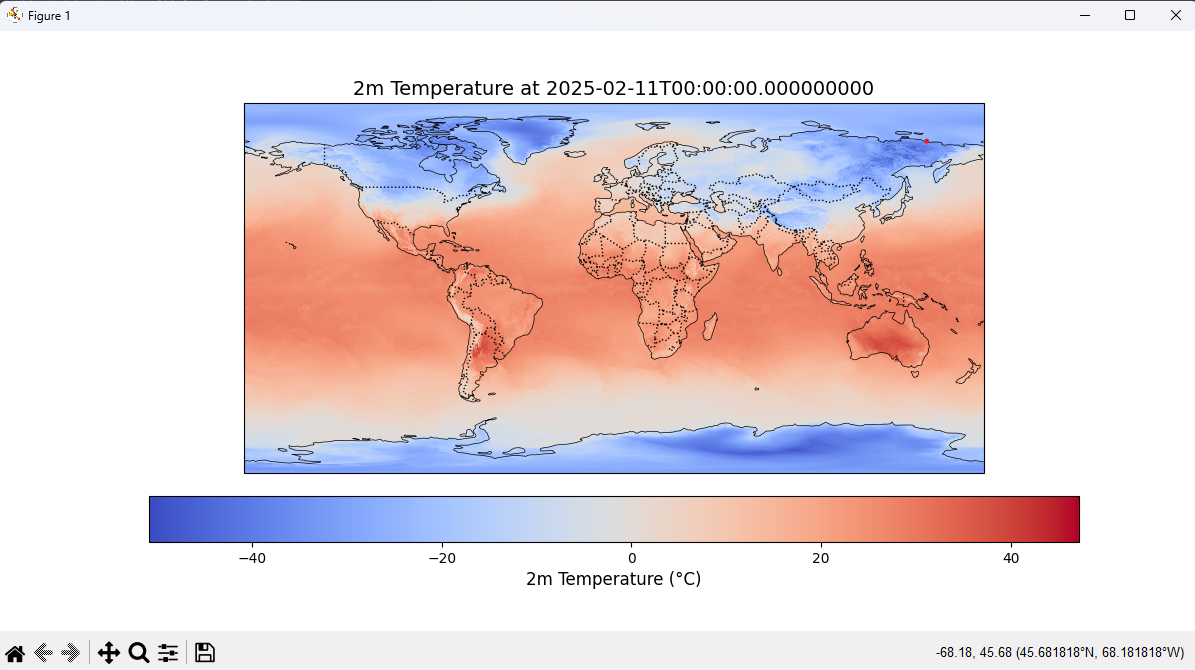
\includegraphics[width=0.85\textwidth]{gif_temp.png}
    \caption{GIF Representation of Temperature Evolution: This animated representation showcases temperature variations over time based on forecast steps. It effectively illustrates how temperature changes across the globe dynamically.}
    \label{fig:gif_temp}
\end{figure}

\textbf{Key Takeaways:}
\begin{itemize}
    \item \textbf{Creates an animated GIF} showing temperature changes over forecast steps.
    \item \textbf{Uses Cartopy} for accurate geospatial projections.
    \item \textbf{Ensures smooth frame transitions} using Matplotlib’s animation API.
\end{itemize}

% ---------------------------------------------------
% 3D Temp Map
% ---------------------------------------------------
\subsection{3D Temperature Map}
\textbf{Goal:} Visualize temperature distribution in 3D to observe spatial trends.

\begin{itemize}
    \item \textbf{Libraries Used:}
    \begin{itemize}
        \item \href{https://matplotlib.org/stable/tutorials/toolkits/mplot3d.html}{Matplotlib 3D} - Creates 3D surface plots.
    \end{itemize}
\end{itemize}

\begin{minted}[
    frame=single, 
    bgcolor=lightgray, 
    fontsize=\footnotesize, 
    breaklines=true, 
    breakanywhere=true
]{python}
from mpl_toolkits.mplot3d import Axes3D
import numpy as np

# Prepare data
t2m_celsius = ds_renamed["t2m"].isel(step=0) - 273.15
t2m_celsius = t2m_celsius.compute()
sorted_indices = np.argsort(ds_renamed.longitude.values)
sorted_longitude = ds_renamed.longitude.values[sorted_indices]

lon, lat = np.meshgrid(sorted_longitude, ds_renamed.latitude.values)
t2m_sorted = t2m_celsius.values[:, sorted_indices]

# Plot 3D surface
fig = plt.figure(figsize=(12, 6))
ax = fig.add_subplot(111, projection='3d')
surf = ax.plot_surface(lon, lat, t2m_sorted, cmap="coolwarm", edgecolor="none")

ax.set_xlabel("Longitude (°)")
ax.set_ylabel("Latitude (°)")
ax.set_zlabel("Temperature (°C)")
ax.set_title("3D Temperature Map")
plt.show()
\end{minted}

\begin{figure}[H]
    \centering
    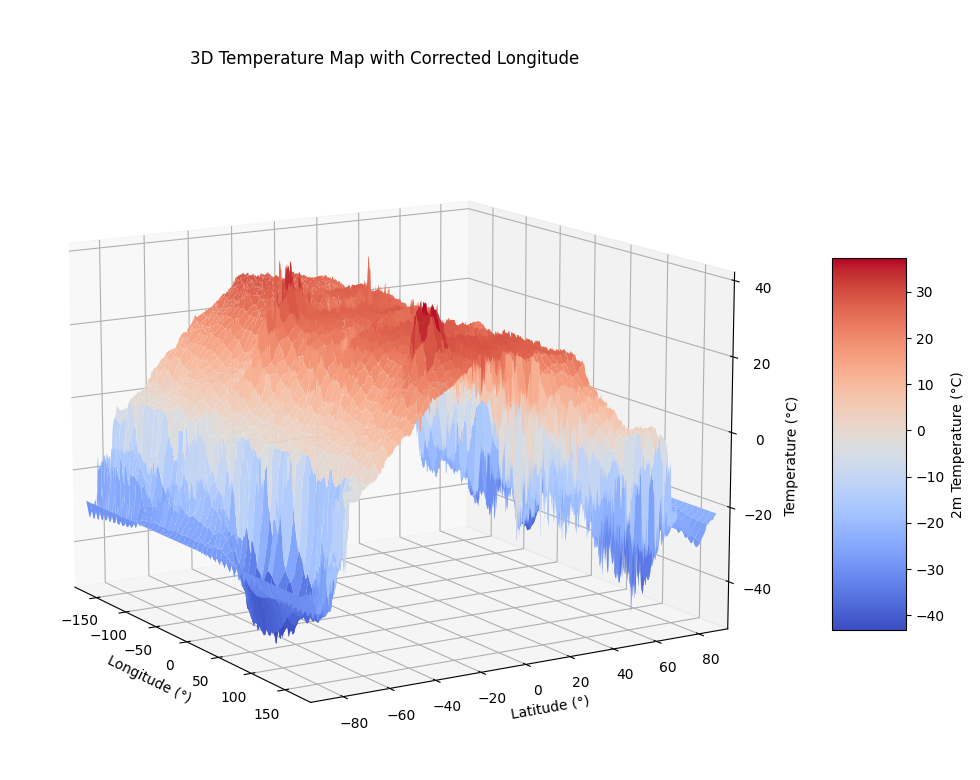
\includegraphics[width=0.739 \textwidth]{3d_map.png}
    \caption{3D Temperature Map: This visualization represents the temperature distribution over a geographical region in a 3D format. The longitude and latitude axes provide spatial reference, while the color gradient from blue to red denotes temperature variations.}
    \label{fig:3d_temp_map}
\end{figure}



\textbf{Key Takeaways:}
\begin{itemize}
    \item \textbf{Visualizes temperature in 3D} to better understand spatial distribution.
    \item \textbf{Uses a color gradient} to highlight temperature variations.
    \item \textbf{Interactive plotting} allows zooming and rotating for deeper analysis.
\end{itemize}

% ---------------------------------------------------
% Converting to Google Earth KML
% ---------------------------------------------------

\begin{center}  
{\color{red} \rule{\linewidth}{1mm} }
\end{center}  
\subsection{Converting to Google Earth KML}
\begin{center}  
{\color{red} \rule{\linewidth}{.1mm}} \
\textbf{\color{white}\colorbox{red}{Needs further investigation about the errors and latency}}  \
\end{center}


\textbf{Goal:} Export meteorological data for visualization in Google Earth.

\begin{itemize}
    \item \textbf{Libraries Used:}
    \begin{itemize}
        \item \href{https://developers.google.com/kml/documentation/}{KML} - Standard format for geospatial visualization.
    \end{itemize}
\end{itemize}

\begin{minted}[
    frame=single, 
    bgcolor=lightgray, 
    fontsize=\footnotesize, 
    breaklines=true, 
    breakanywhere=true
]{python}
# Define KML header
kml_header = """<?xml version="1.0" encoding="UTF-8"?>
<kml xmlns="http://www.opengis.net/kml/2.2">
<Document>
"""

# Generate KML Placemarks with colored temperature markers
kml_body = ""
for lat in ds_renamed.latitude.values[::5]:  
    for lon in ds_renamed.longitude.values[::5]:
        temp_value = ds_renamed["t2m"].isel(latitude=lat, longitude=lon).values - 273.15
        kml_body += f"""
<Placemark>
  <name>{temp_value:.1f}°C</name>
  <Point>
    <coordinates>{lon},{lat},0</coordinates>
  </Point>
</Placemark>
"""

# Close KML file
kml_footer = """</Document></kml>"""

# Save KML file
with open("temperature_data.kml", "w") as file:
    file.write(kml_header + kml_body + kml_footer)
\end{minted}

\newpage
\subsection{KML File Rendering Issue}

While attempting to visualize temperature data in Google Earth, an issue was encountered where the labels appear overly dense, overlapping each other, making it difficult to interpret.

\begin{figure}[H]
    \centering
    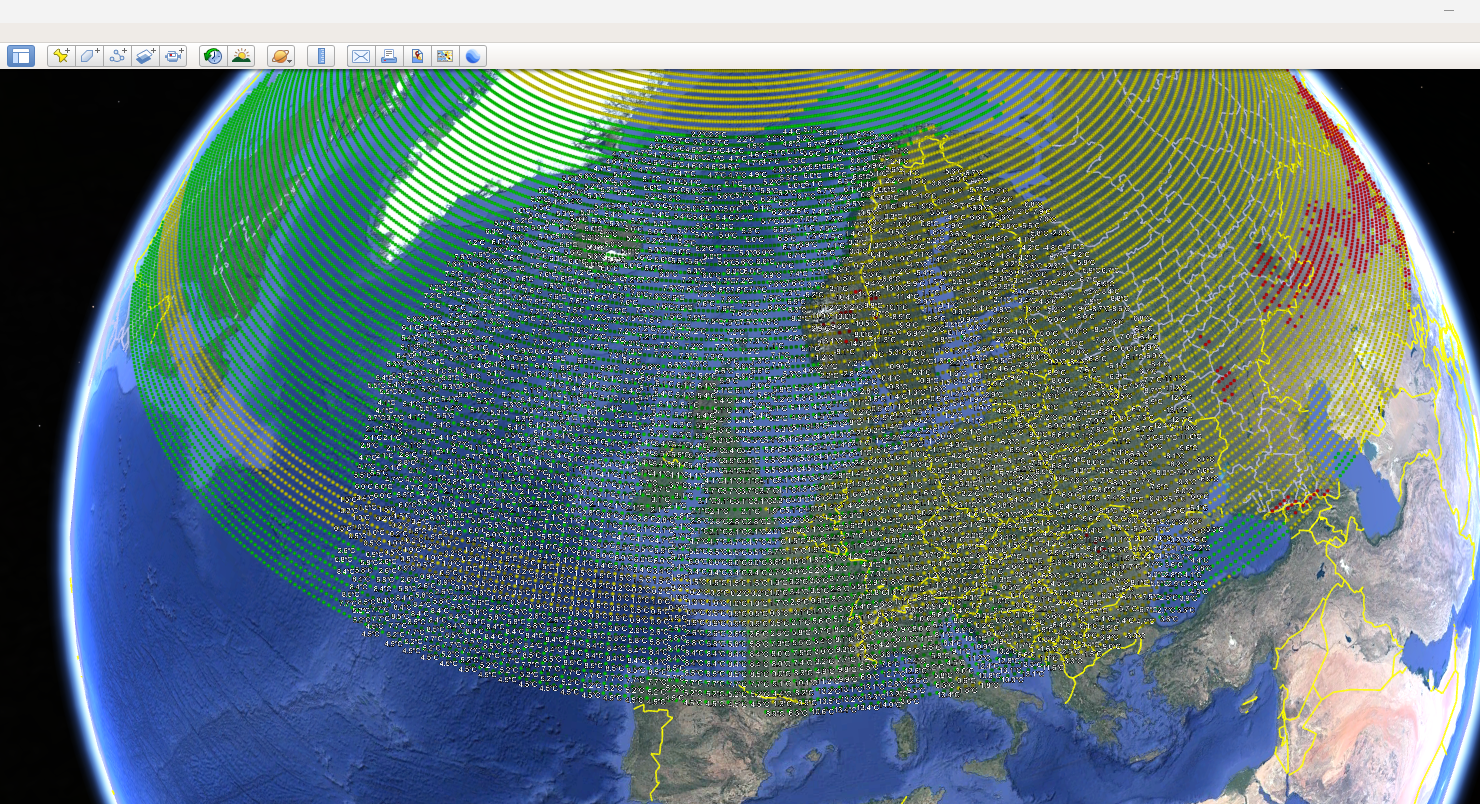
\includegraphics[width=0.9\textwidth]{gge_image_error.png}
    \caption{Google Earth KML Visualization Error: The temperature labels are excessively dense, leading to cluttered rendering. The KML file requires adjustments to improve readability.}
    \label{fig:kml_error}
\end{figure}

\subsection{Explanation of Error}

The visualization issue in Figure \ref{fig:kml_error} occurs due to the **high density of temperature data points**. This results in:
\begin{itemize}
    \item \textbf{Overlapping Labels:} The values are positioned too closely, making them unreadable.
    \item \textbf{Excessive Data Points:} The dataset might be **too high resolution** for practical visualization.
    \item \textbf{Lack of Spacing Adjustment:} There is no filtering to reduce the number of displayed points.
    \item \textbf{Suboptimal Rendering in Google Earth:} The current settings do not adapt well to a **large number of labels**.
\end{itemize}

\subsection{Possible Fixes}

To improve the KML visualization and make it more readable, we propose the following solutions:

\begin{enumerate}
    \item \textbf{Reduce Data Density:} Display only every $n$th data point to prevent excessive labels.
    \item \textbf{Improve Label Formatting:} Modify text sizes, transparency, or spacing in the KML generation script.
    \item \textbf{Use Clustered Data Representation:} Instead of individual points, group temperature values into a **regional average**.
    \item \textbf{Increase Point Spacing:} Modify how latitude and longitude values are processed in the KML script.
\end{enumerate}

By implementing these fixes, the visualization in **Google Earth** will be significantly improved, allowing for better insights into temperature distributions. \\

\textbf{Key Takeaways:}
\begin{itemize}
    \item \textbf{Converts meteorological data to KML format} for Google Earth visualization.
    \item \textbf{Creates temperature markers} at different locations.
    \item \textbf{Allows real-time interaction} with temperature data in a 3D environment.
\end{itemize}

\end{document}


